\chapter{Personas}

Für die Implementierung des Moduls haben wir folgende Personas entwickelt:

\section{Persona A: Charlie Blomquist}

\begin{figure}[H]
	\centering
	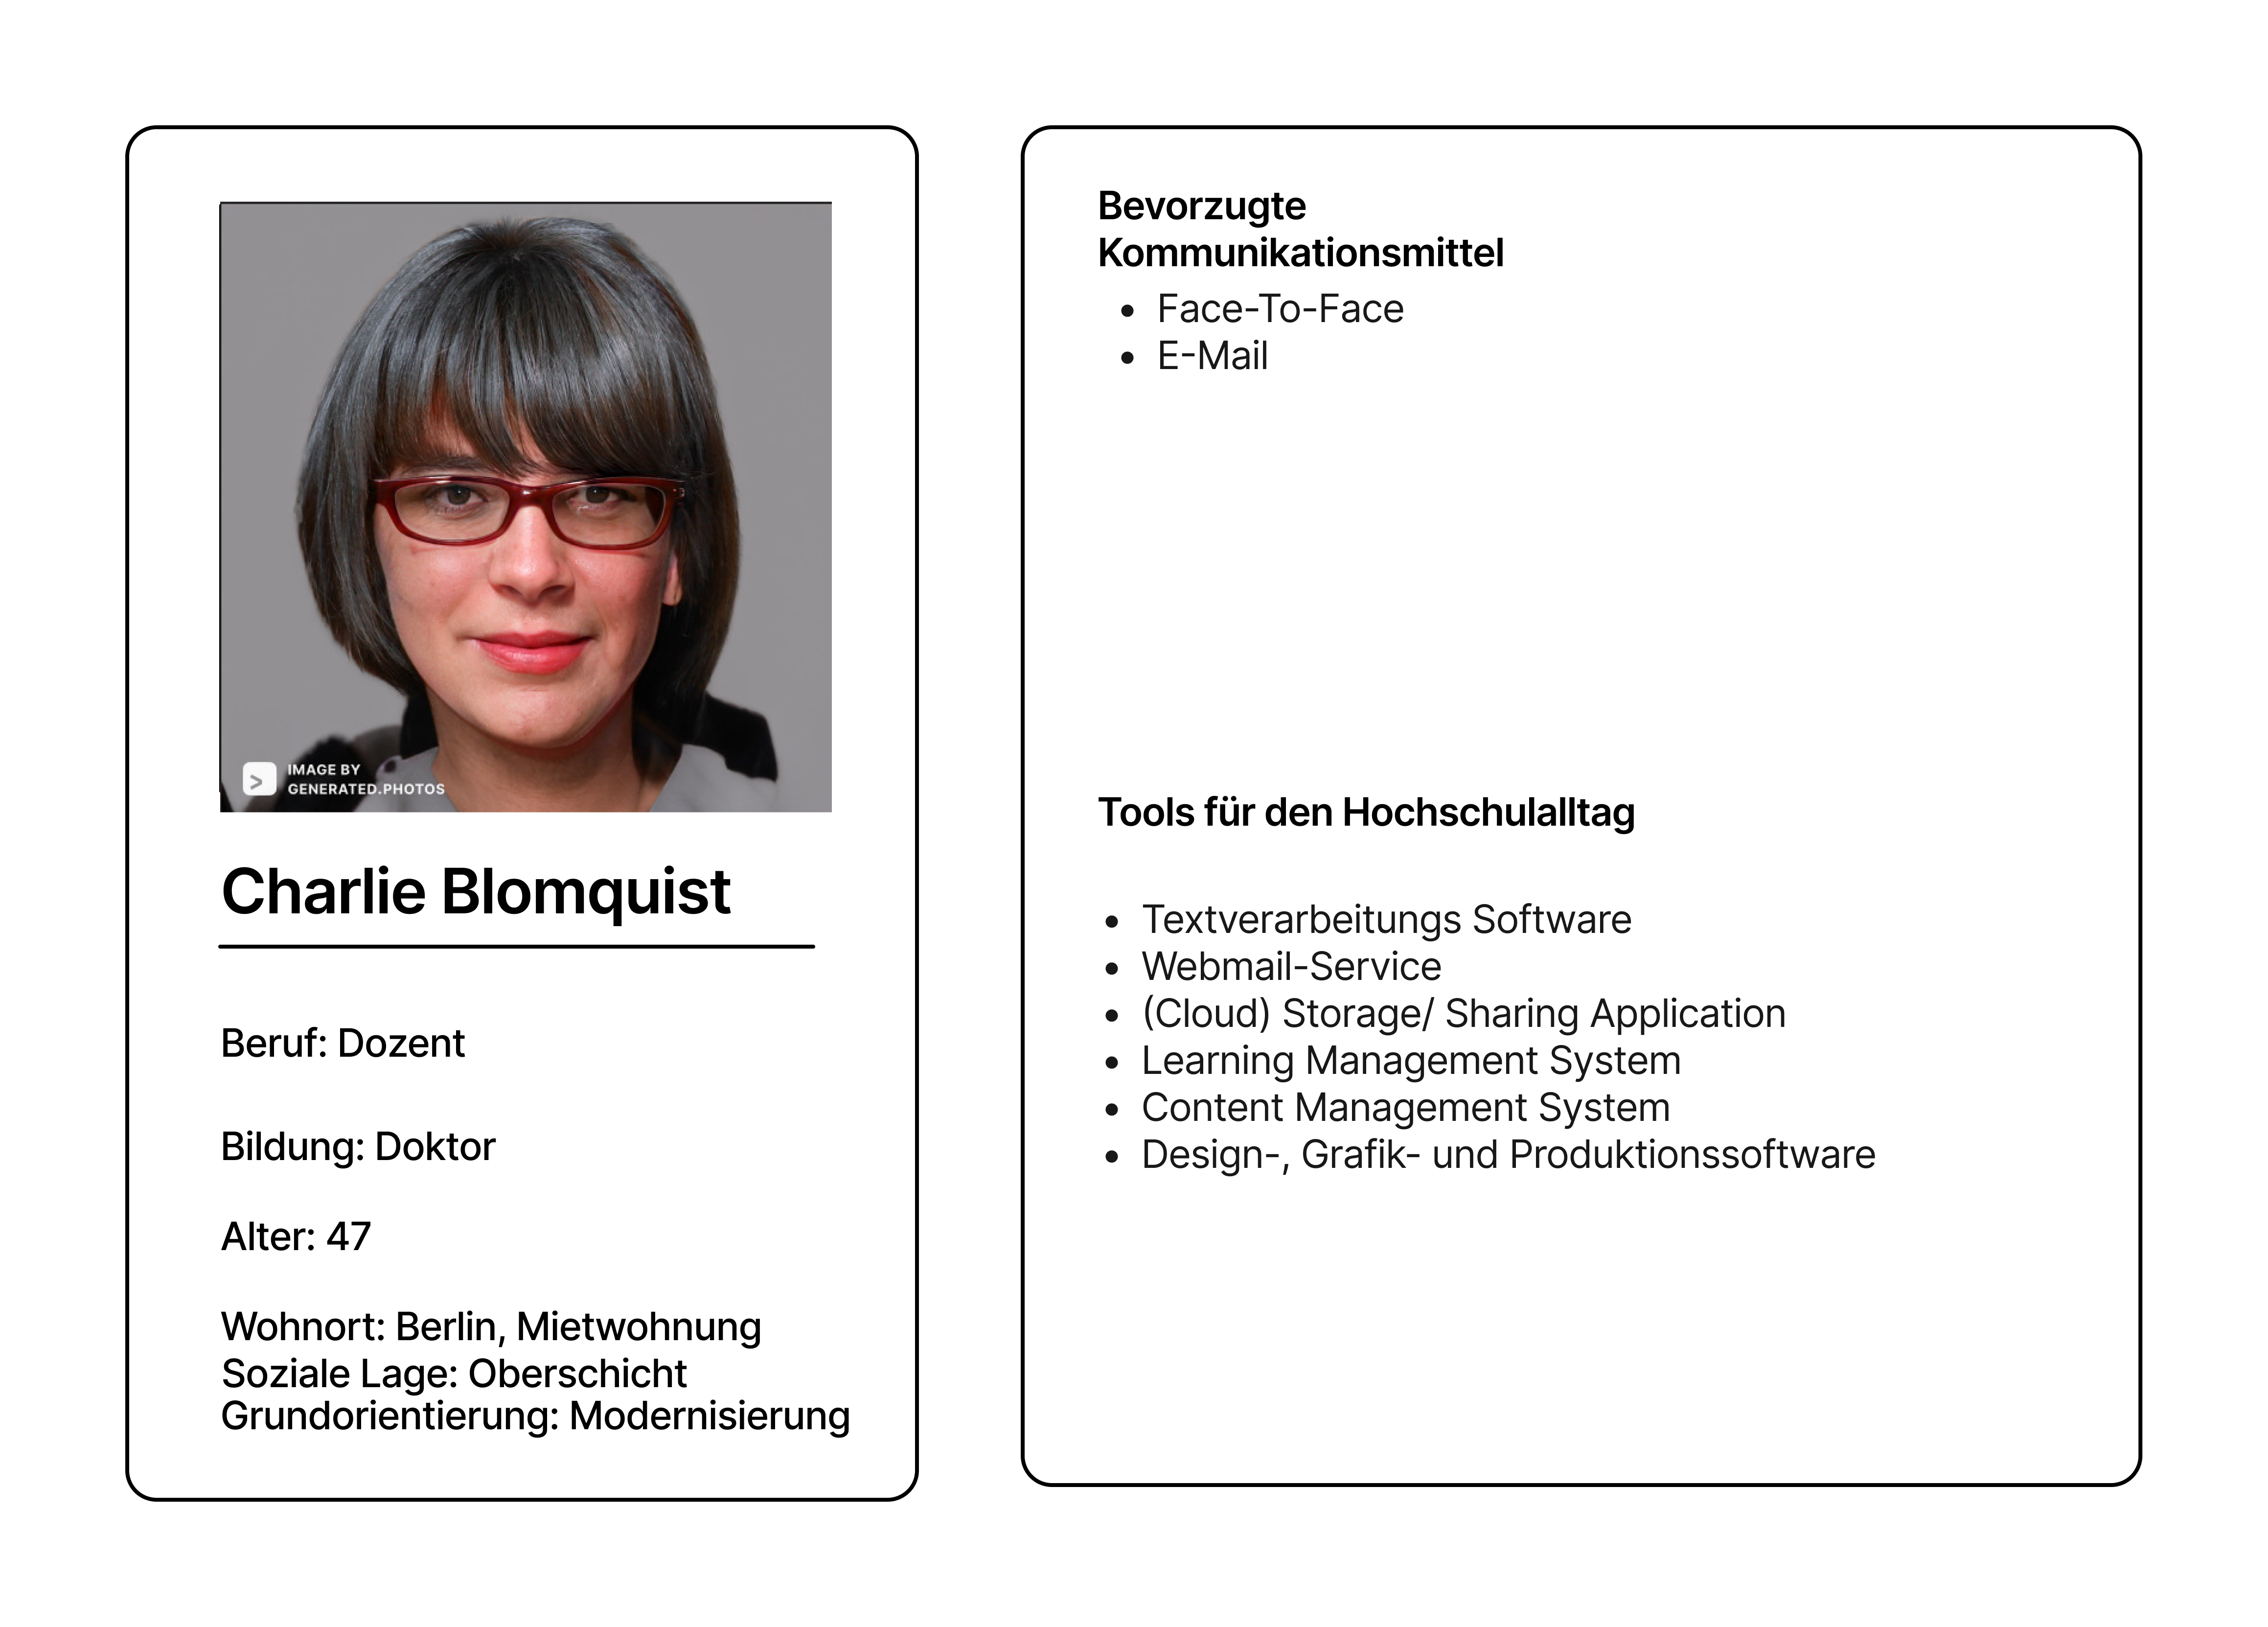
\includegraphics[width=0.95\textwidth]{persona-a-overview.png}
    \caption{Kurzvorstellung Charlie Blomquist}
	\label{fig:personaashort}
\end{figure}

\begin{figure}[H]
	\centering
	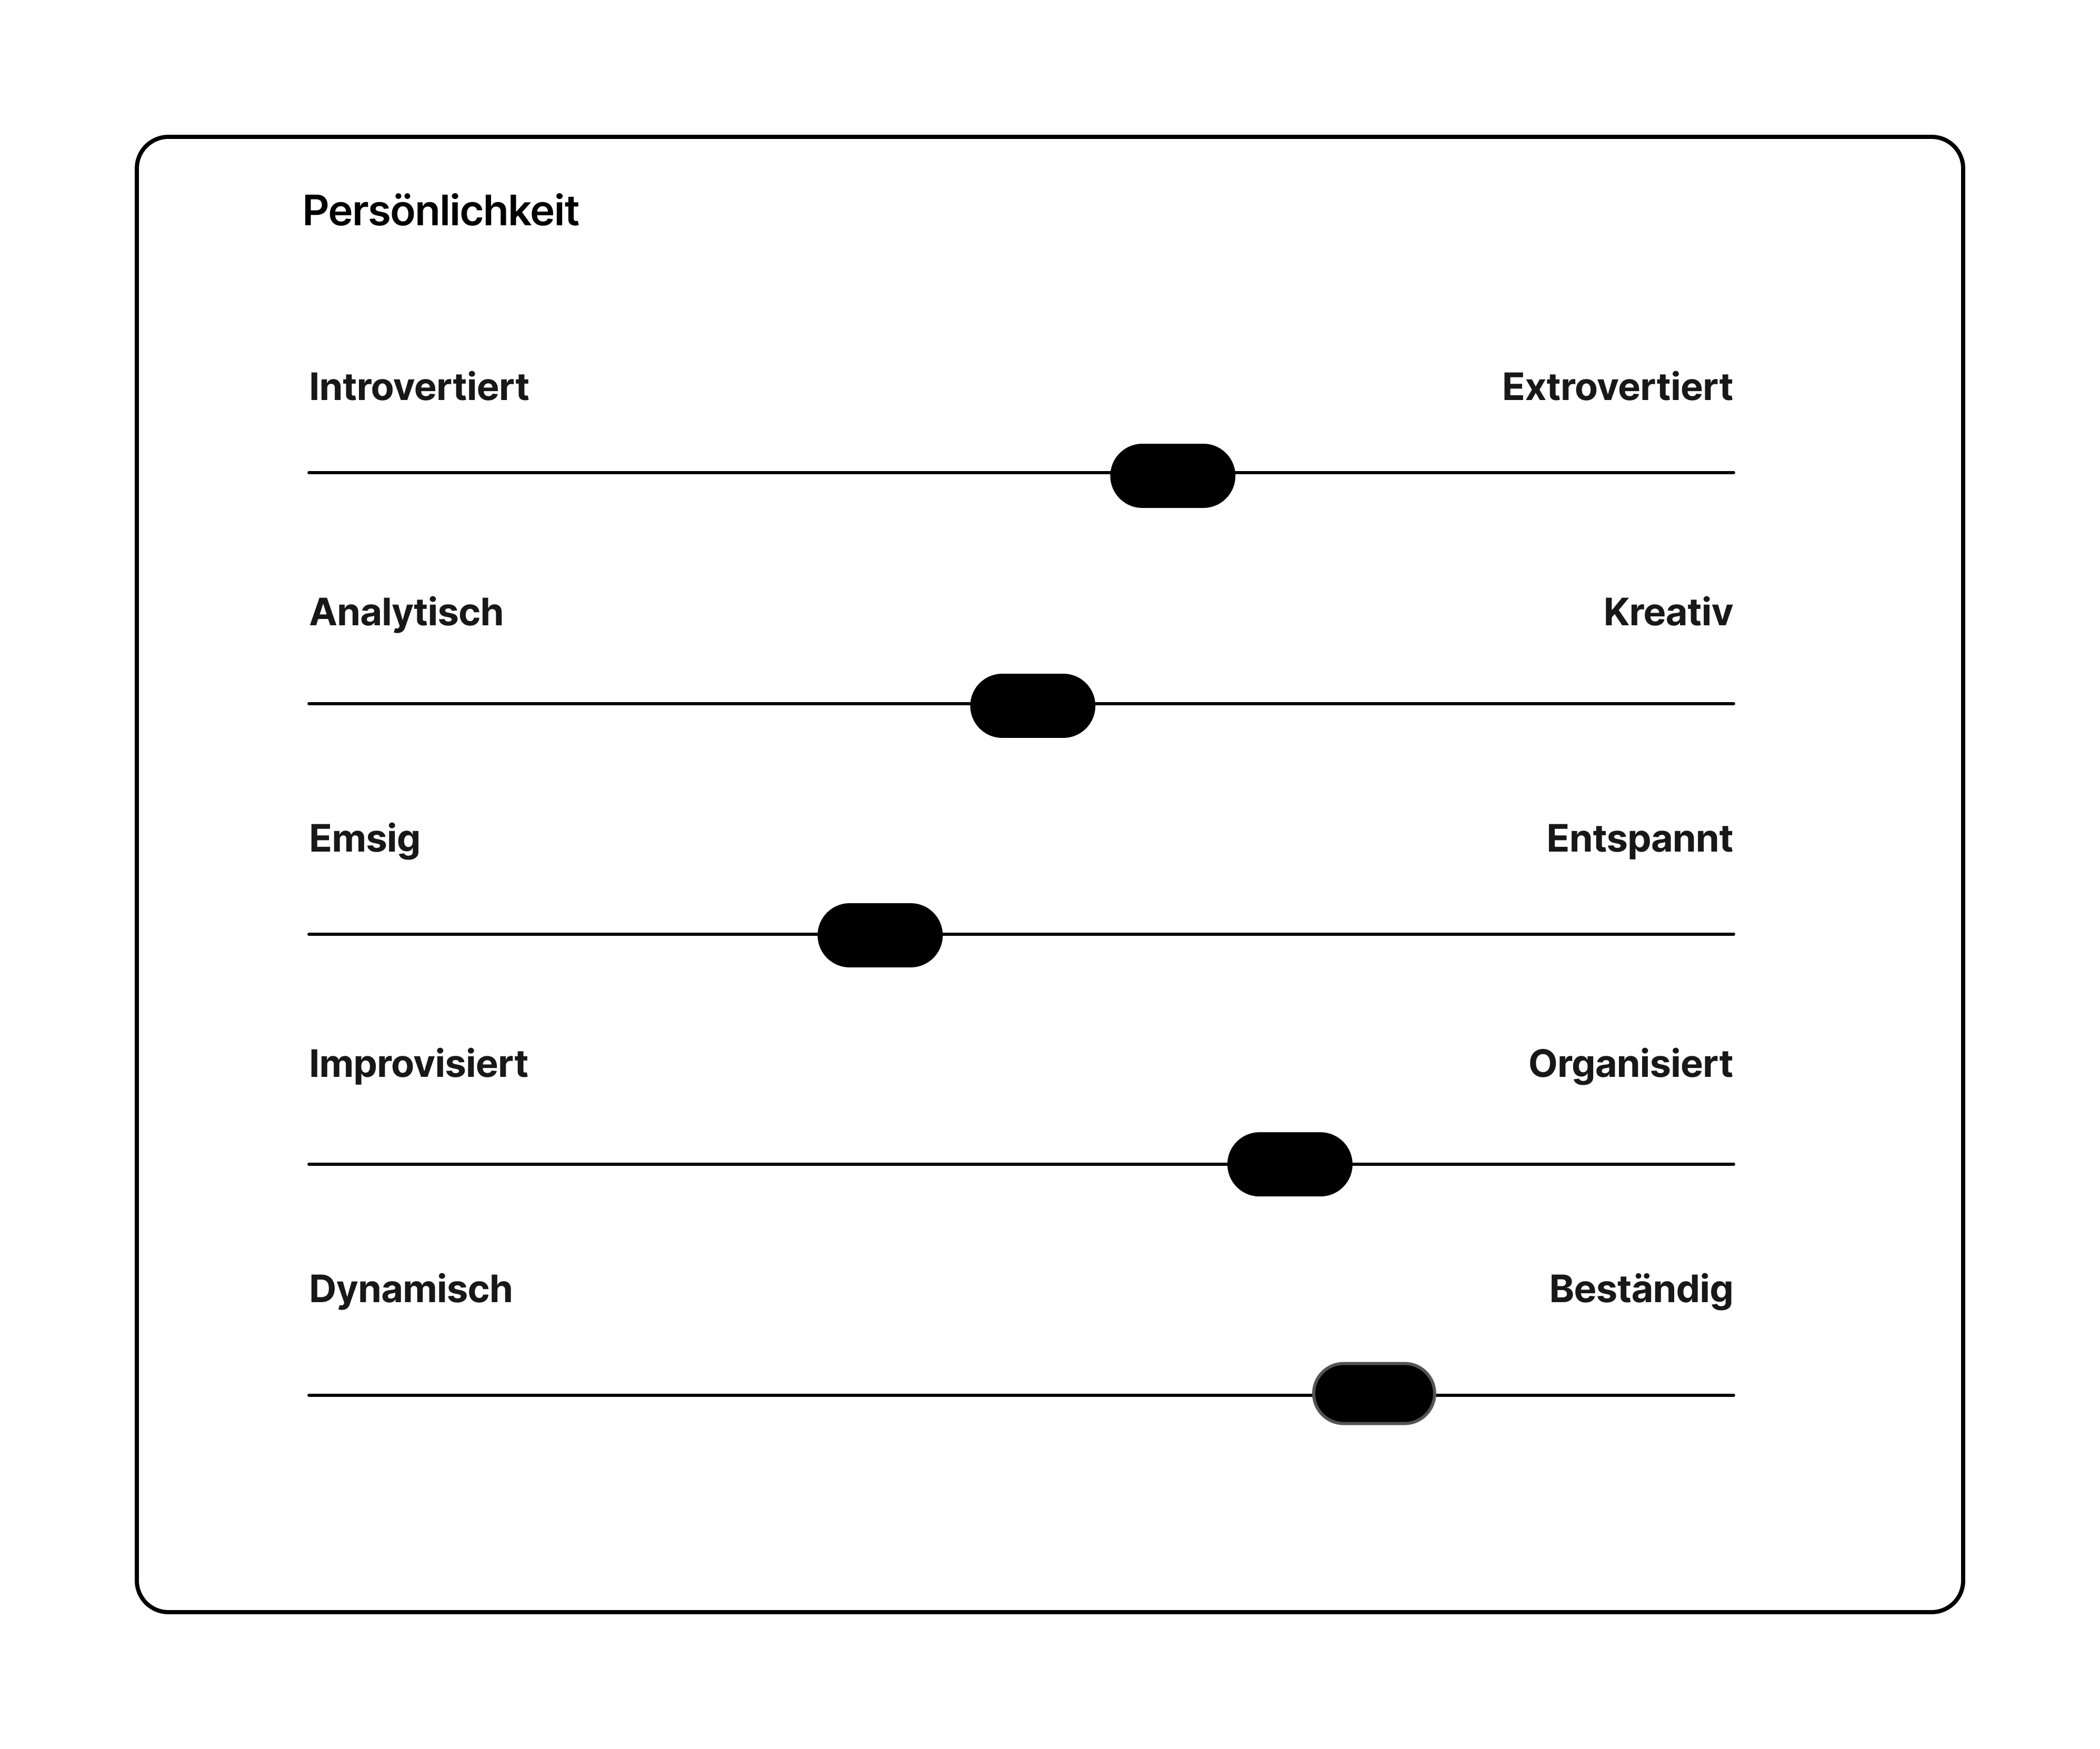
\includegraphics[width=0.95\textwidth]{persona-a-personality.png}
    \caption{Persönlichkeitszüge von Charlie Blomquist}
	\label{fig:personaapers}
\end{figure}

\begin{figure}[H]
	\centering
	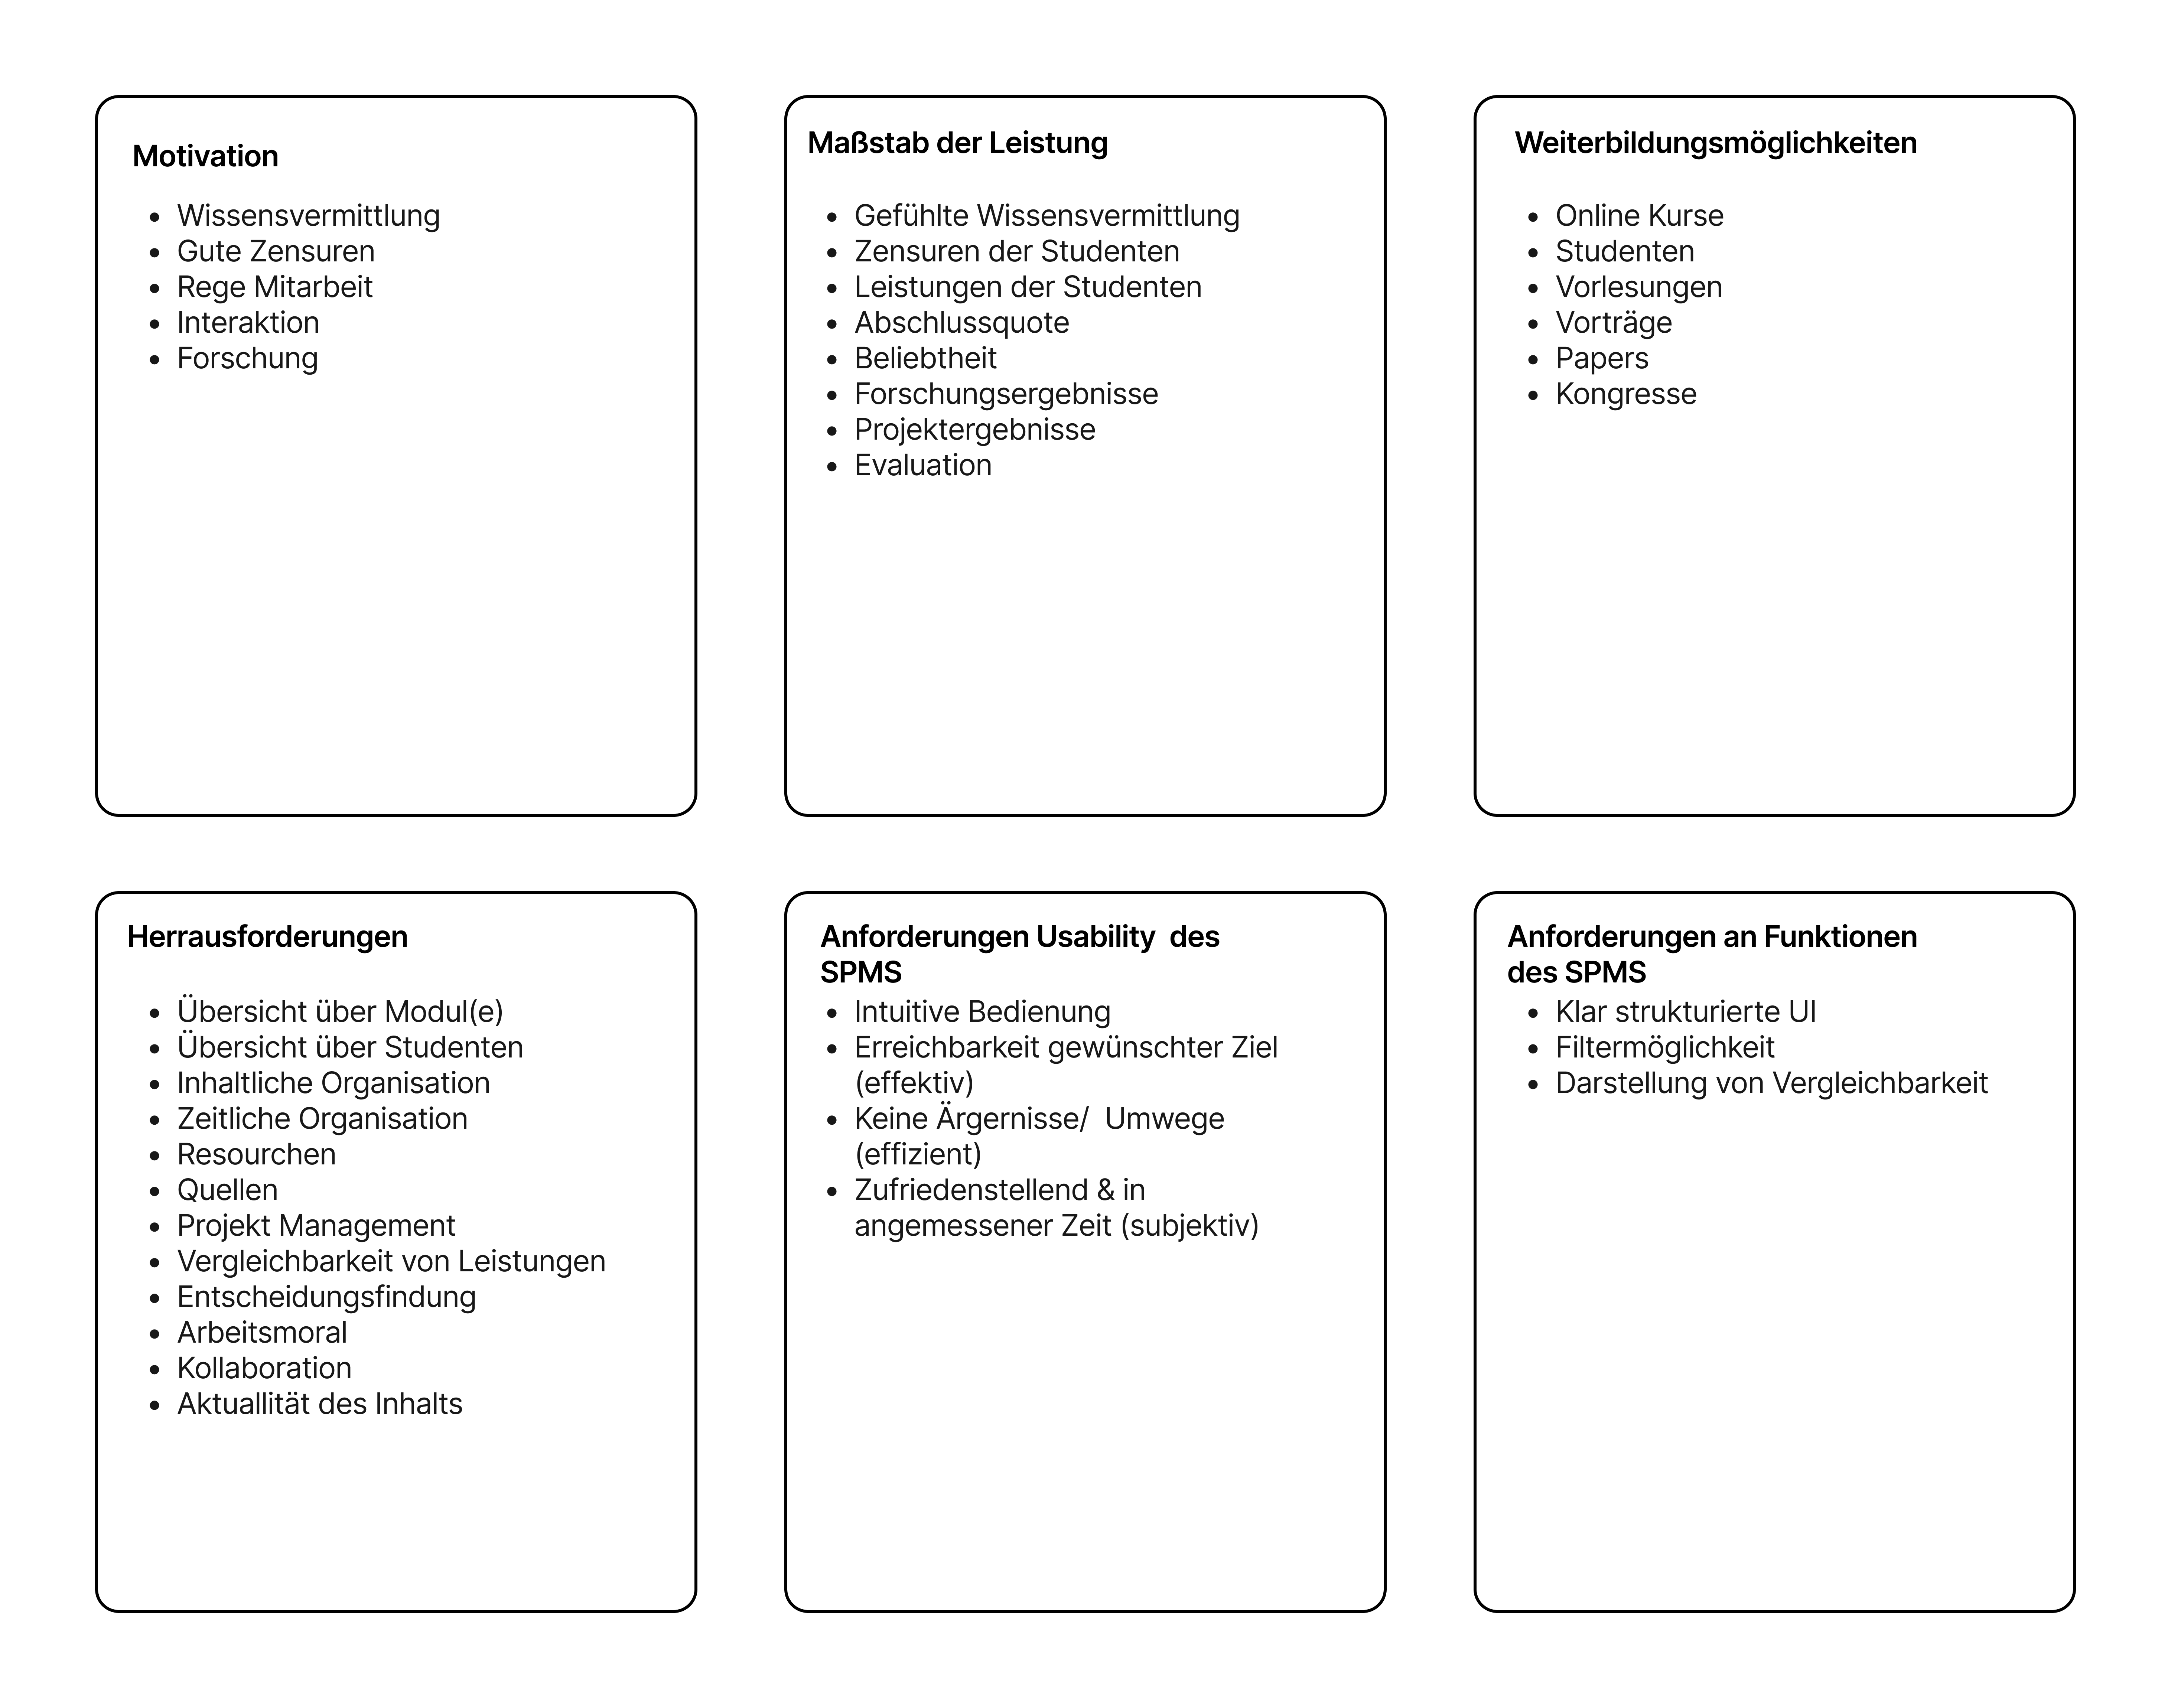
\includegraphics[width=0.95\textwidth]{persona-a-further.png}
    \caption{Weitere Informationen zu Chalie Blomquist}
	\label{fig:personaafurther}
\end{figure}

\section{Persona B: Kai Lind}

\begin{figure}[H]
	\centering
	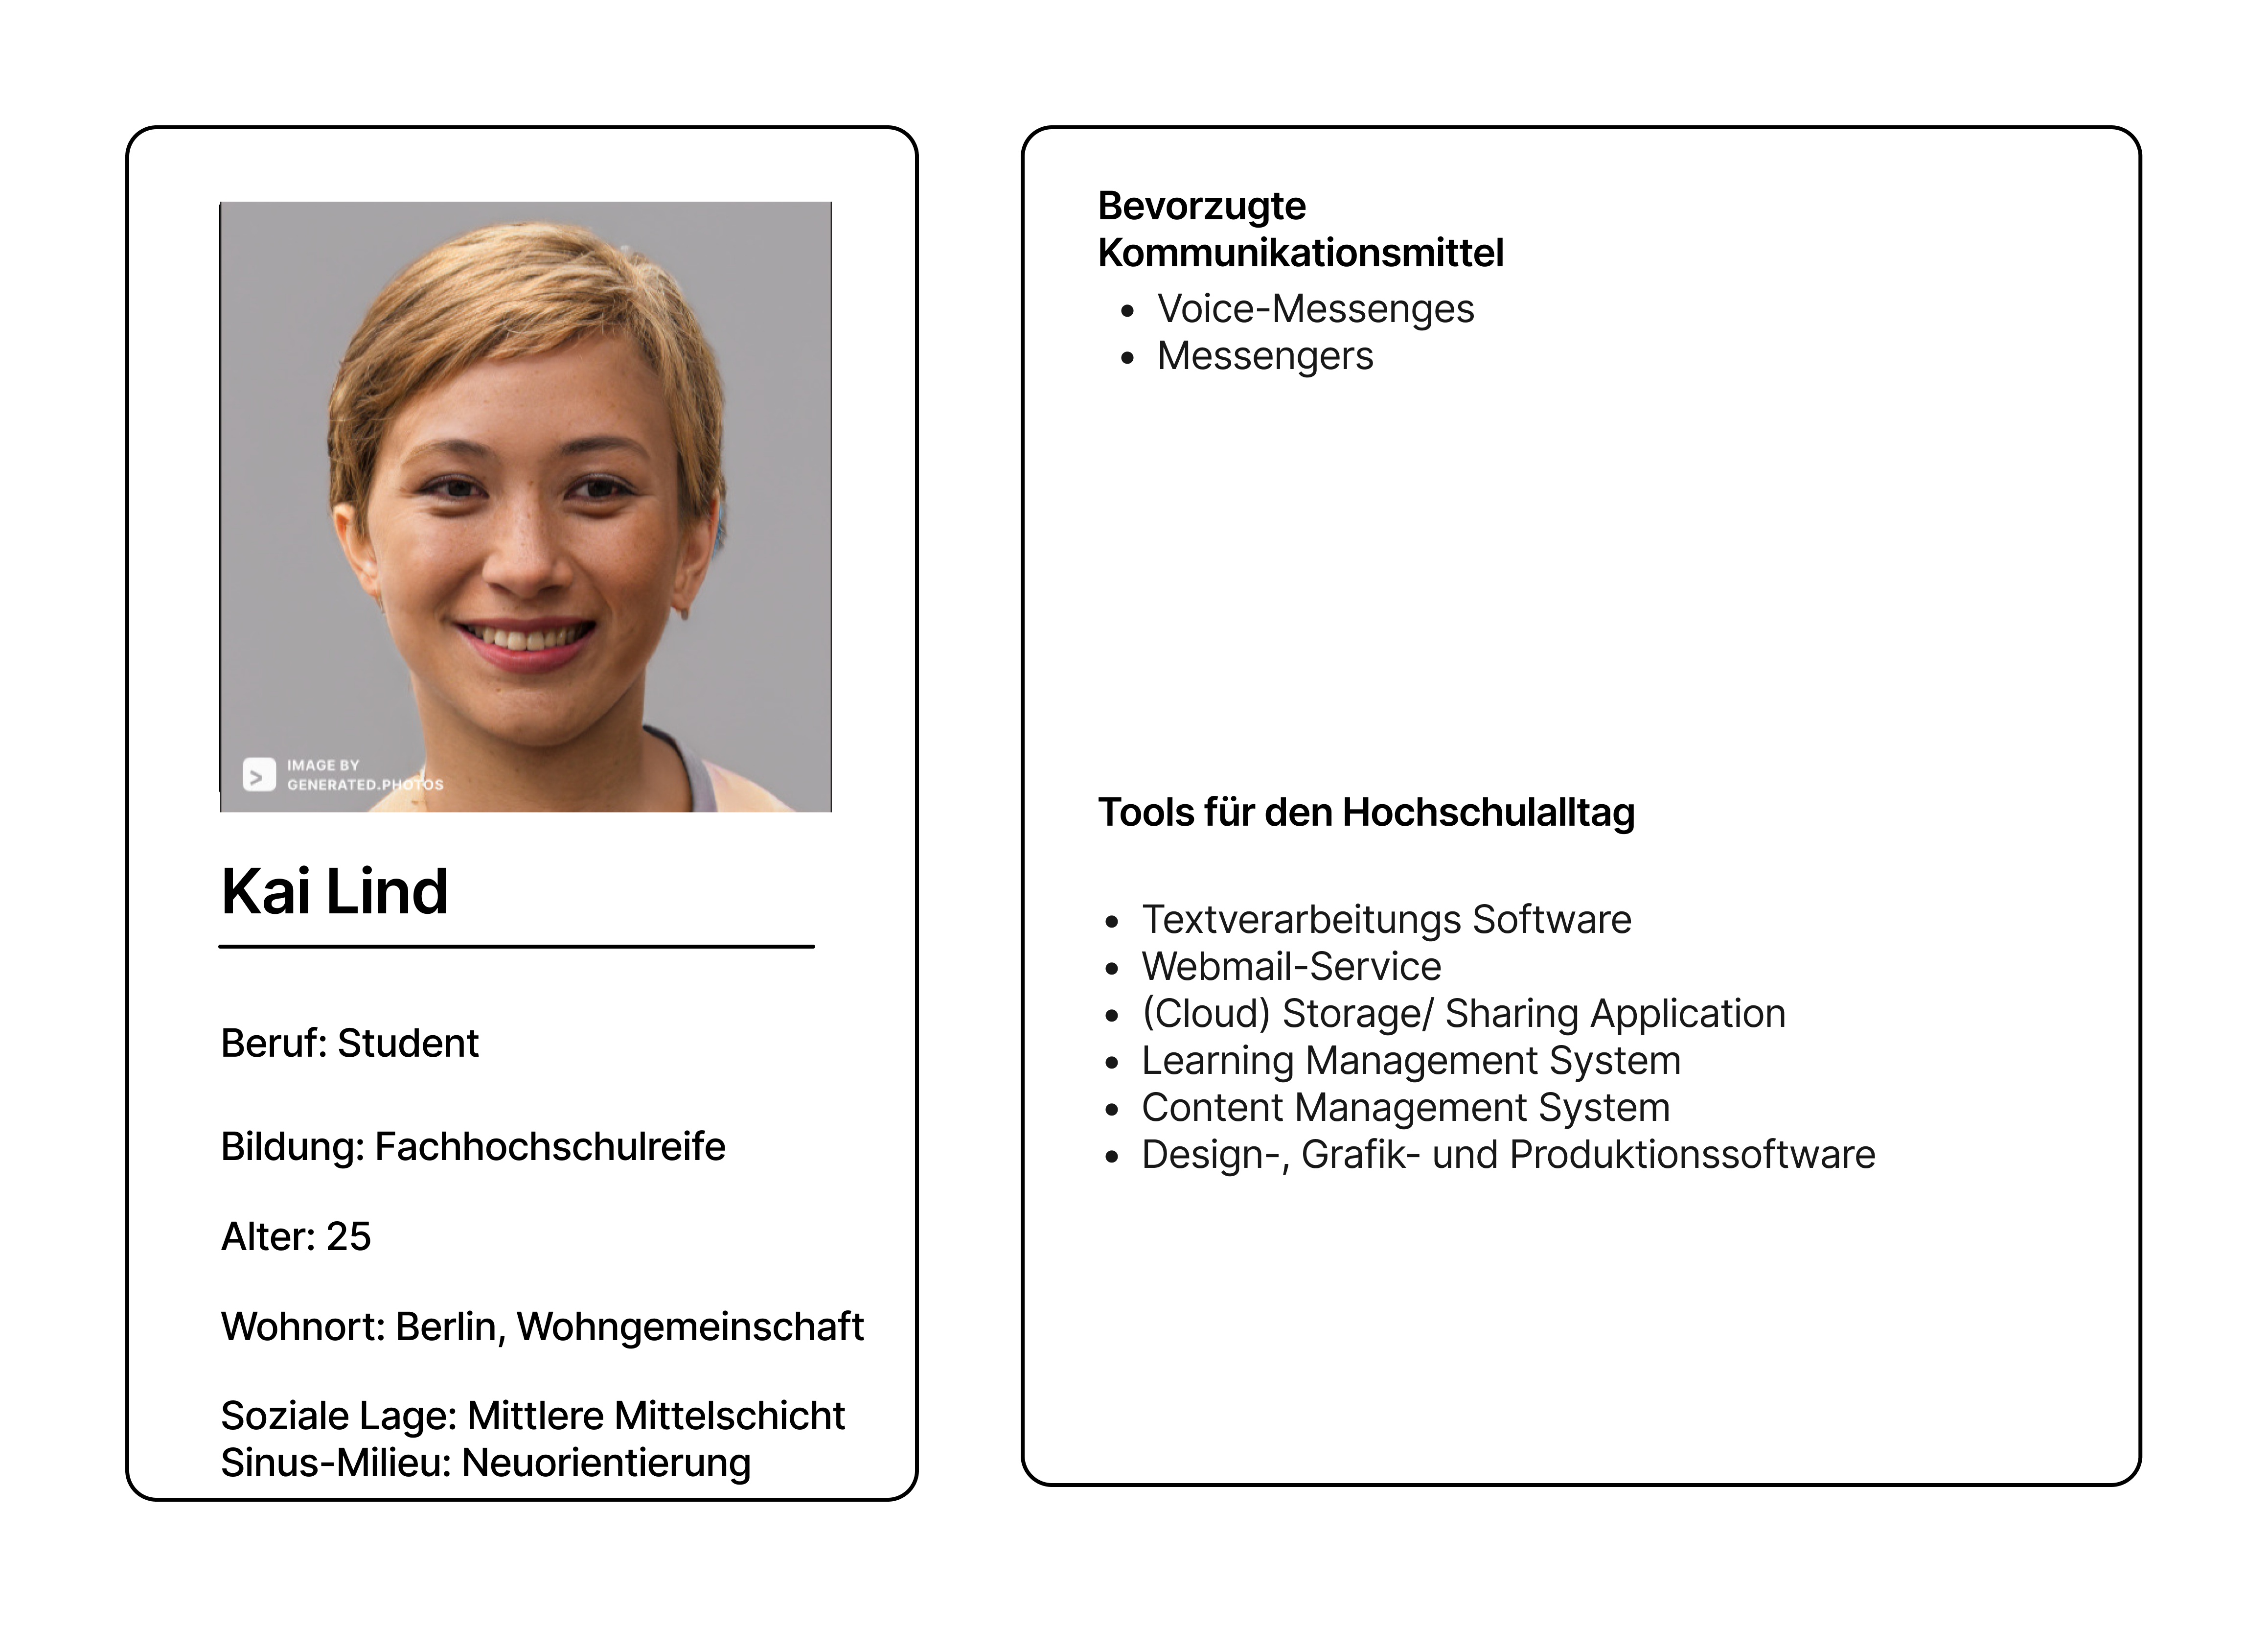
\includegraphics[width=0.95\textwidth]{persona-b-overview.png}
    \caption{Kurzvorstellung Kai Lind}
	\label{fig:personabshort}
\end{figure}

\begin{figure}[H]
	\centering
	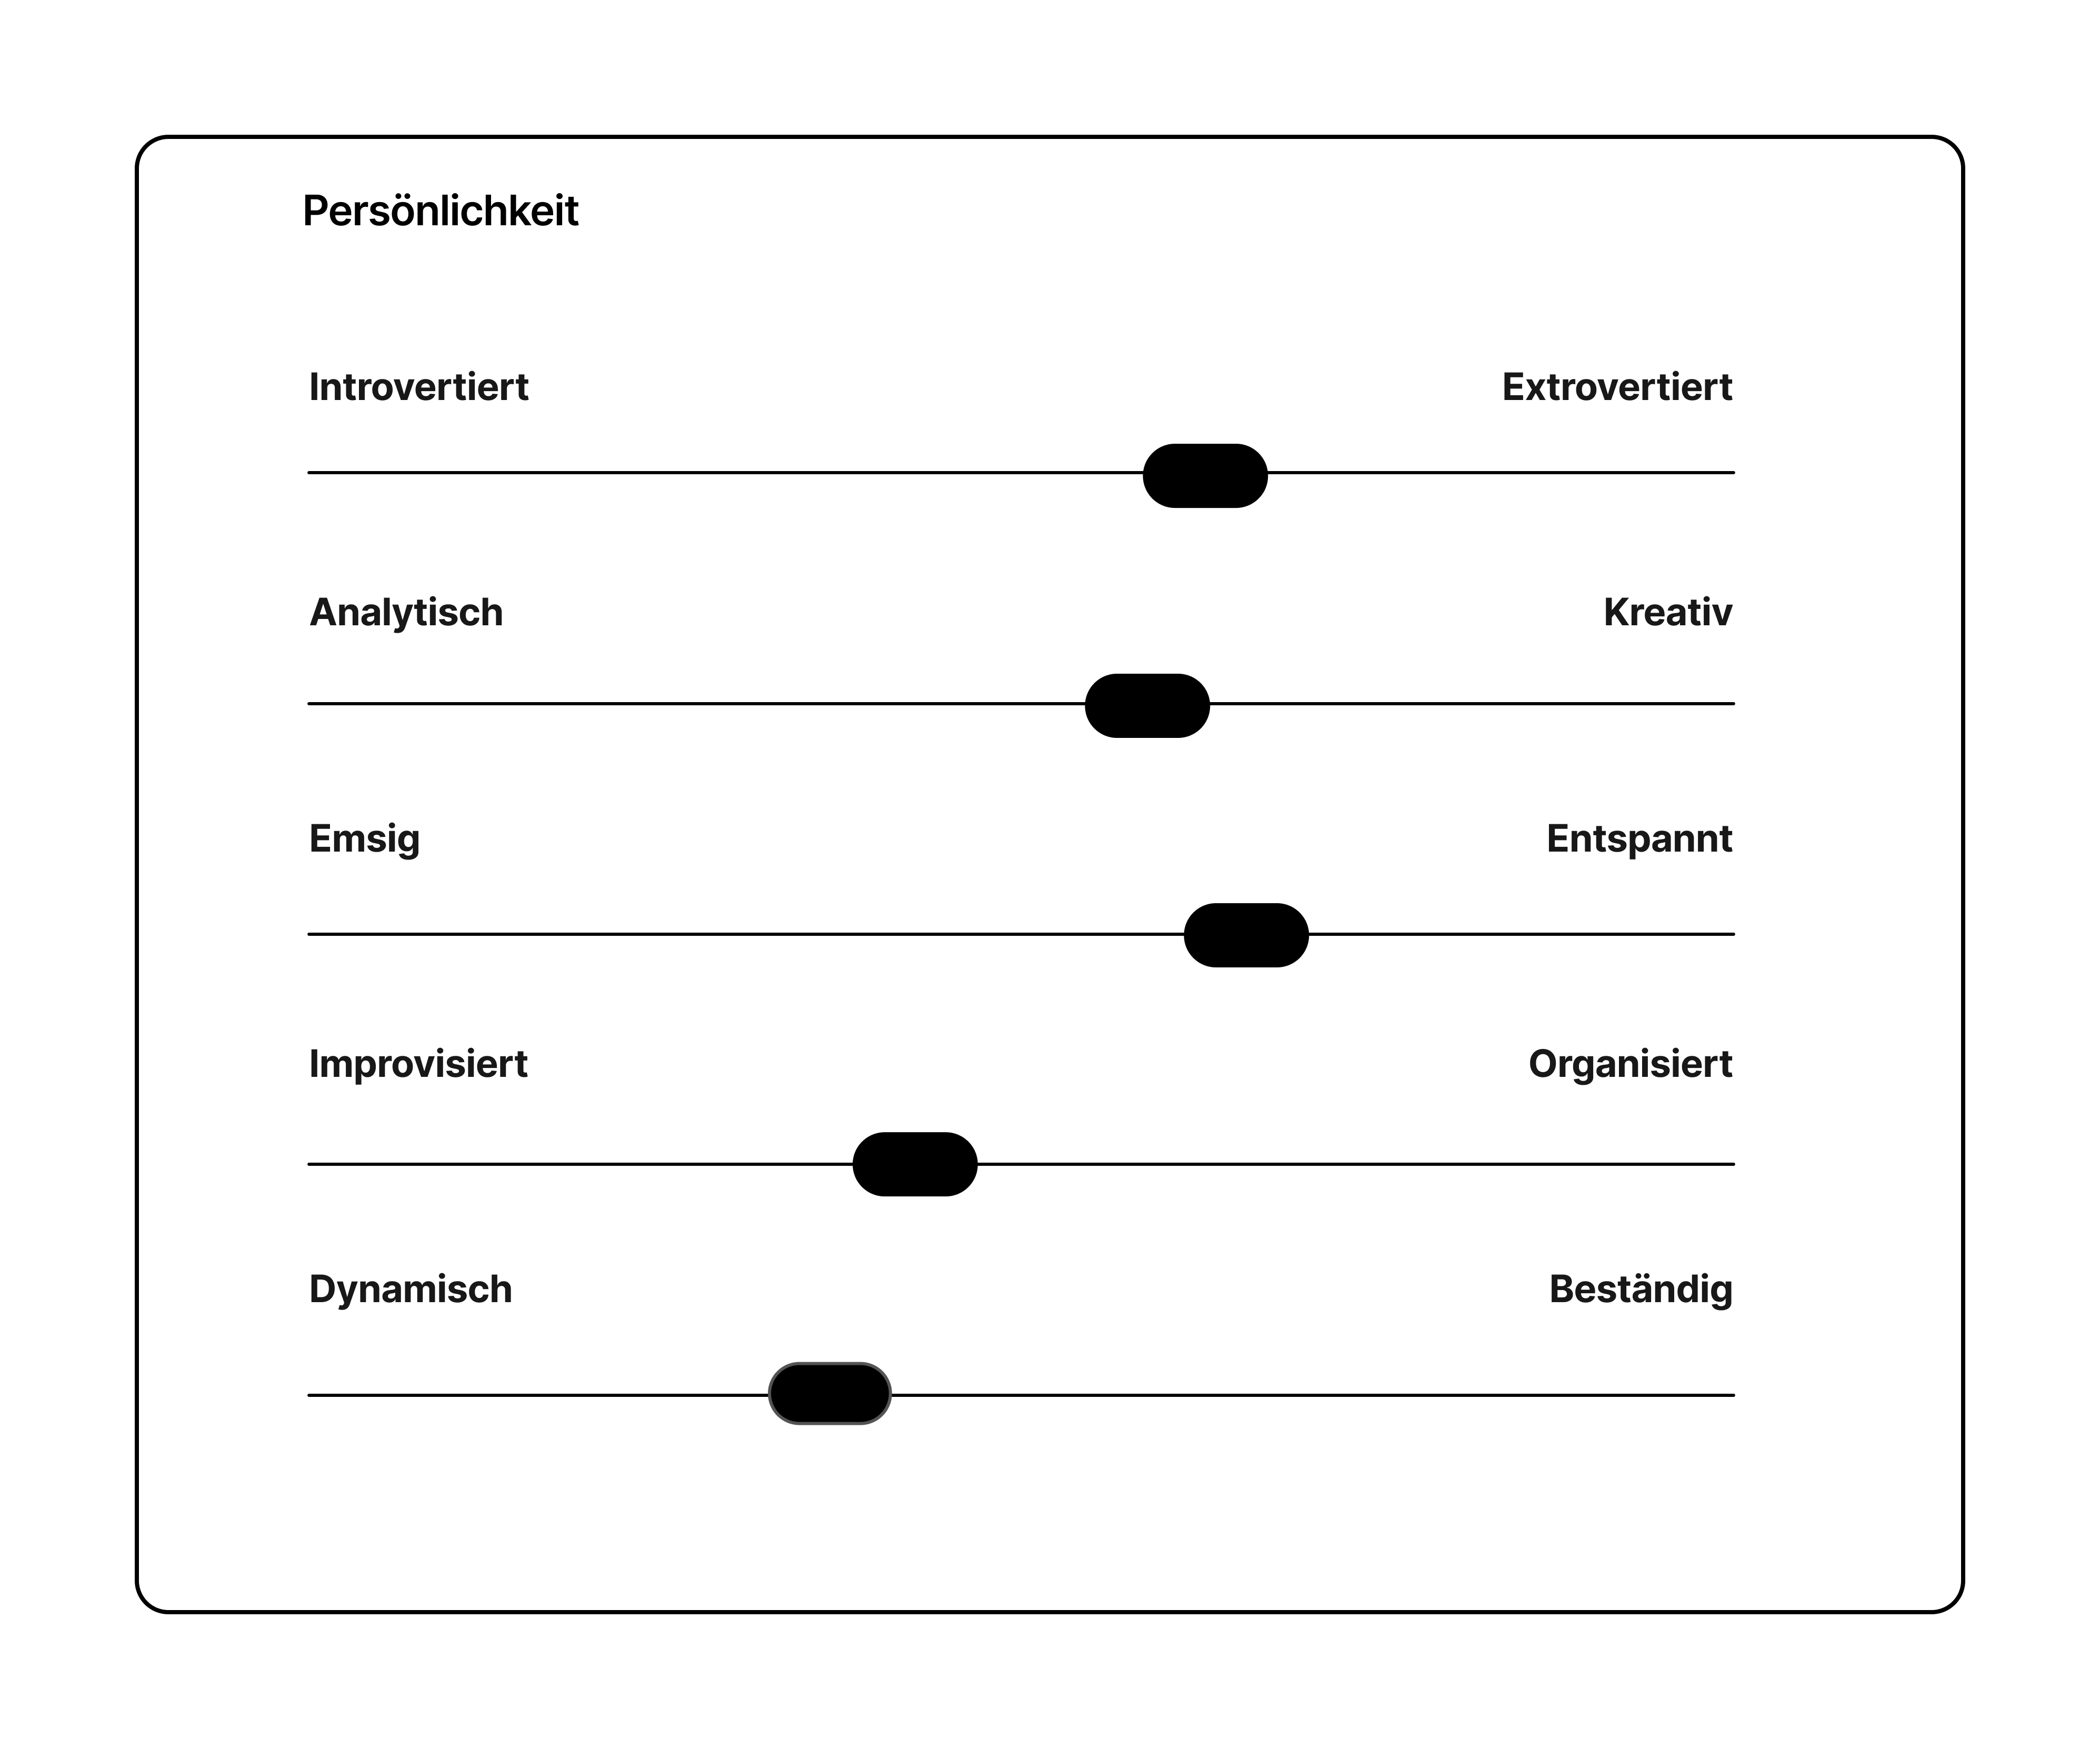
\includegraphics[width=0.95\textwidth]{persona-b-personality.png}
    \caption{Persönlichkeitszüge von Kai Lind}
	\label{fig:personabpers}
\end{figure}

\begin{figure}[H]
	\centering
	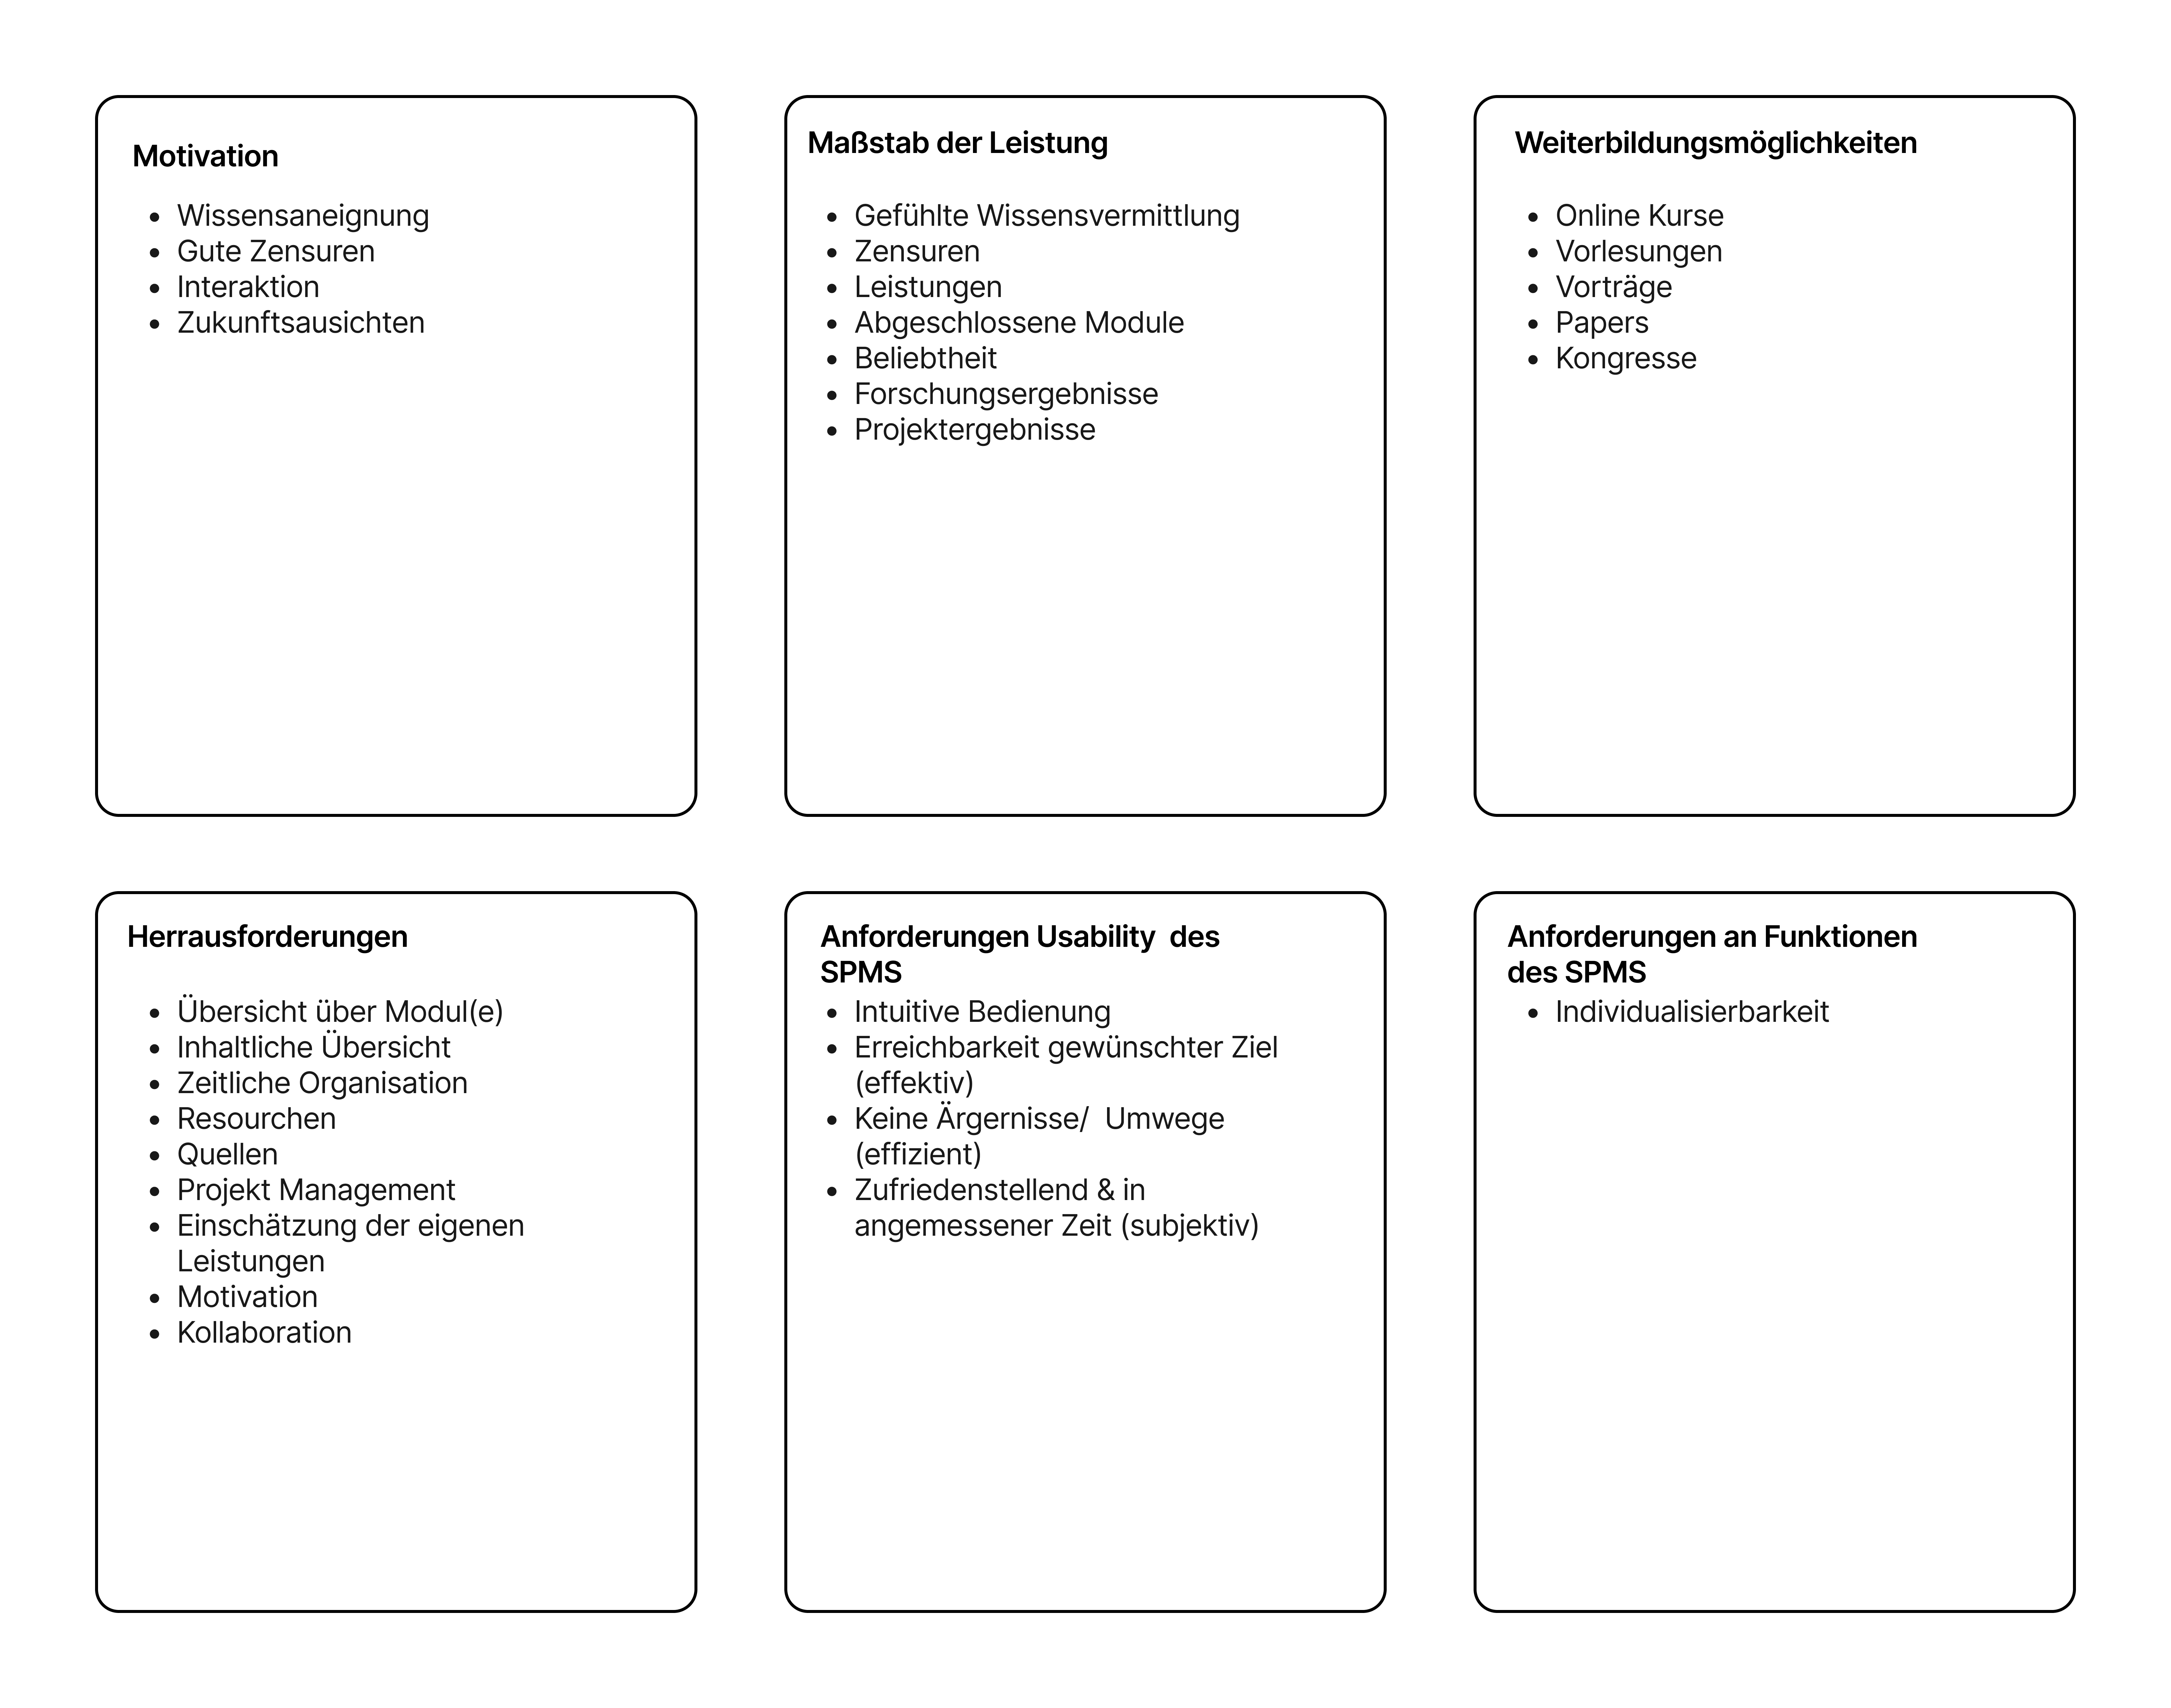
\includegraphics[width=0.95\textwidth]{persona-b-further.png}
    \caption{Weitere Informationen zu Kai Lind}
	\label{fig:personabfurther}
\end{figure}


\section{Hintergrund zu Personas}

Personas sind, im Bereich \ac{MCI}, ein häufig genutztes Mittel im Anforderungsmanagement um die Zielgruppe einer Anwendung genauer zu definieren\cite{inproceedings}. Sie dienen dazu während des Designprozesses Motivationen und Bedürfnisse möglicher Nutzer besser zu antizipieren und frühzeitig zu berücksichtigen.
Die von uns erarbeiteten Personas entsprechen in weiten Teilen den von uns erwarteten Zielnutzern. Hierfür haben wir uns einen durchschnittlichen \cite{dzhw2018} Studenten sowie einen durchschnittlichen Dozenten \cite{statista2021} erarbeitet.

